\documentclass[11pt,a4paper]{article}
\usepackage[T1]{fontenc}
\usepackage[utf8]{inputenc}
\usepackage{tgtermes}
\usepackage[margin=2.5cm,top=2.4cm,bottom=2.6cm]{geometry}
\usepackage{graphicx,booktabs,xcolor,caption,amsmath,float}
\usepackage{microtype}
\usepackage[hidelinks]{hyperref}

\definecolor{ecink}{HTML}{1A2430}
\definecolor{ecgray}{HTML}{5A6572}
\captionsetup{font={small},labelsep=period,
              justification=justified,singlelinecheck=false}
\setlength{\parskip}{5pt}\setlength{\parindent}{0pt}
\color{ecink}
\newcommand{\fignote}[1]{\par\vspace{4pt}%
  \begin{minipage}{\linewidth}\footnotesize\color{ecgray}#1\end{minipage}}
\newcommand{\starlegend}{\\[2pt]
\hspace*{0pt}***Significant at the 1 percent level.\\
\hspace*{0pt}\phantom{*}**Significant at the 5 percent level.\\
\hspace*{0pt}\phantom{**}*Significant at the 10 percent level.}

\begin{document}

\begin{center}
{\fontsize{17}{22}\selectfont\bfseries
Who Leaves Teaching, and Why?\par}
\vspace{4pt}
{\fontsize{12.5}{16}\selectfont
The Anatomy of Teacher Attrition in the United States, 1997--2024\par}
\vspace{10pt}
{\small José Elías Durán Roa \quad\textcolor{ecgray}{University of
Alicante and OECD}}\par
\vspace{2pt}
{\small\textcolor{ecgray}{Figures and appendix material \quad July 2026}}
\end{center}
\vspace{6pt}

% ================= main figures =================
\begin{figure}[H]
\centering
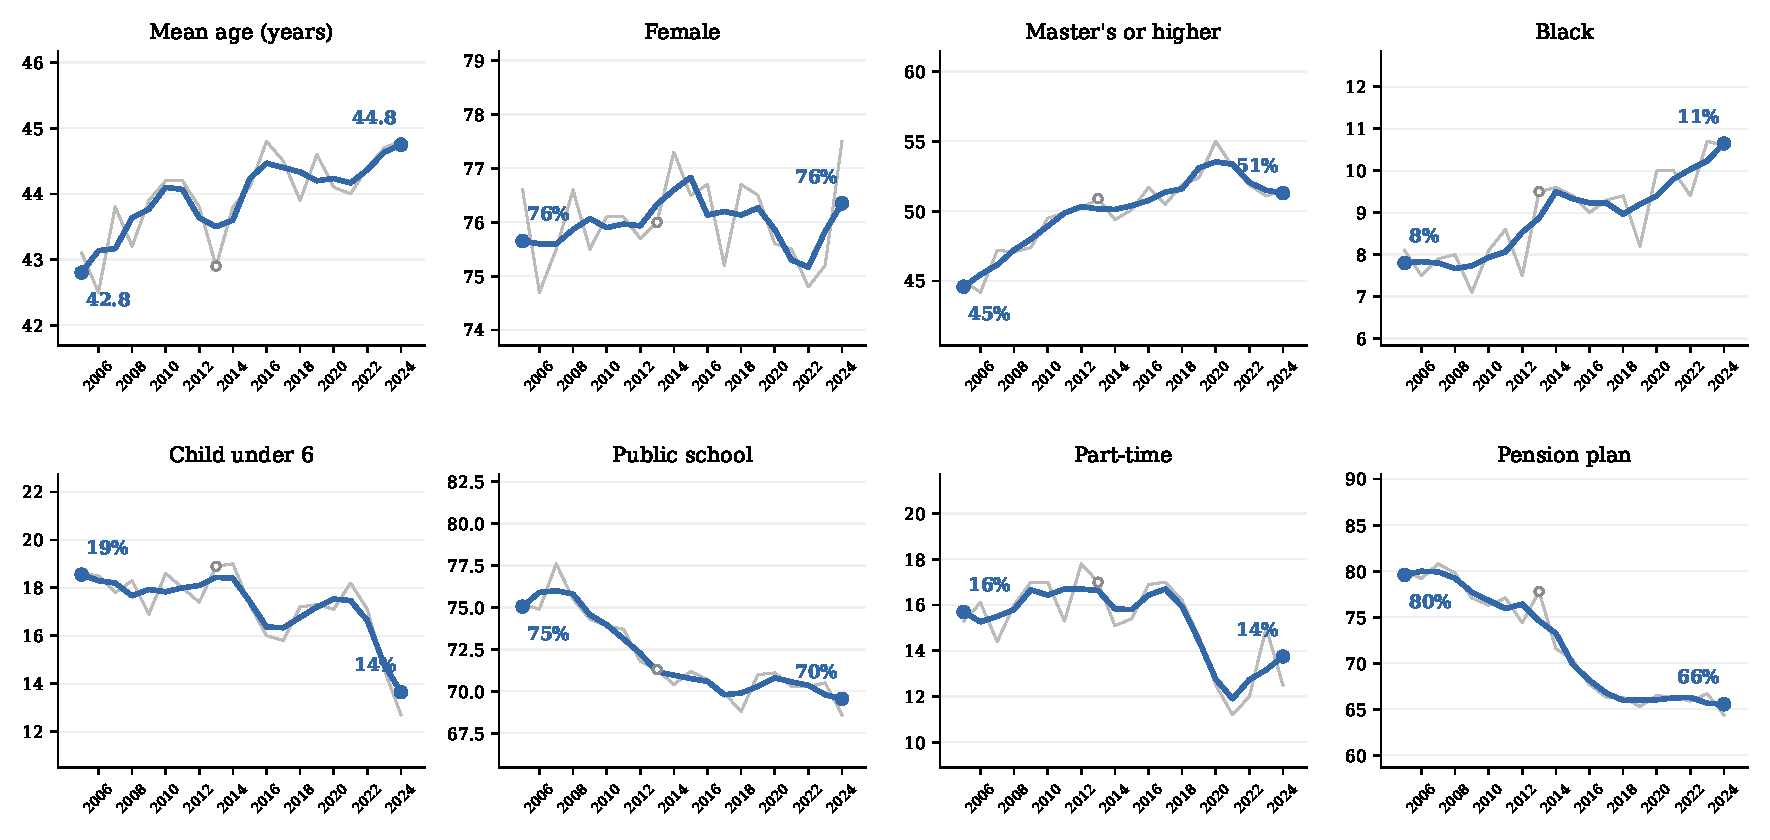
\includegraphics[width=\linewidth]{figures/g1_workforce.pdf}
\caption{Composition of the Teaching Workforce, 2005--2024}
\fignote{\textit{Notes:} College-graduate teachers aged 18+ whose
longest job last year was K--12 teaching; ASEC supplement weights.
Thin gray lines are annual values; blue lines are centered 3-year
averages, with endpoint values printed. ``Public school,''
``part-time,'' and ``pension plan'' refer to the longest job held last
year; the open circle marks 2013, a year with a reduced sample due to
the ASEC redesign. \textit{Source:} Author's calculations from March
CPS supplements, survey years 2006--2025.}
\end{figure}
\clearpage

\begin{figure}[H]
\centering
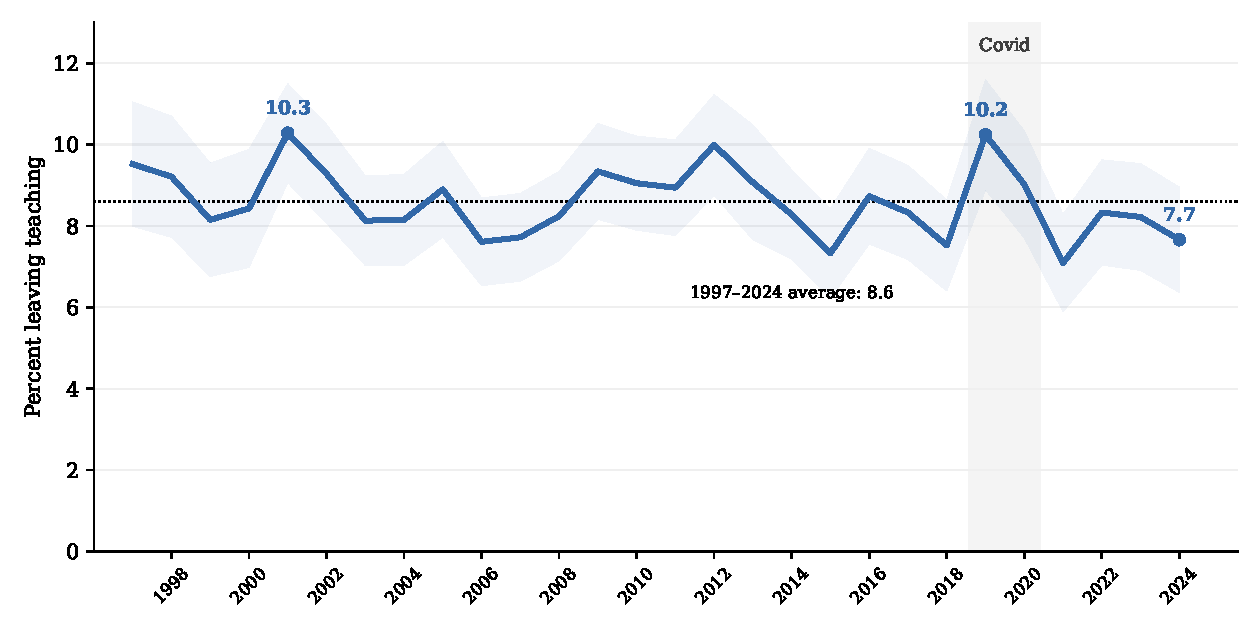
\includegraphics[width=0.92\linewidth]{figures/g2_evolution.pdf}
\caption{Leaving Teaching, 1997--2024}
\fignote{\textit{Notes:} Share of college-graduate teachers (longest
job last calendar year) not employed in a teaching occupation the
following March, by route-based definition; ASEC weights. Shaded band:
95 percent confidence interval using a design factor of 1.5. Dotted
line: the 1997--2024 mean (8.6). The gray band marks the Covid
supplements. \textit{Source:} Author's calculations from March CPS
supplements, survey years 1998--2025.}
\end{figure}
\clearpage

\begin{figure}[H]
\centering
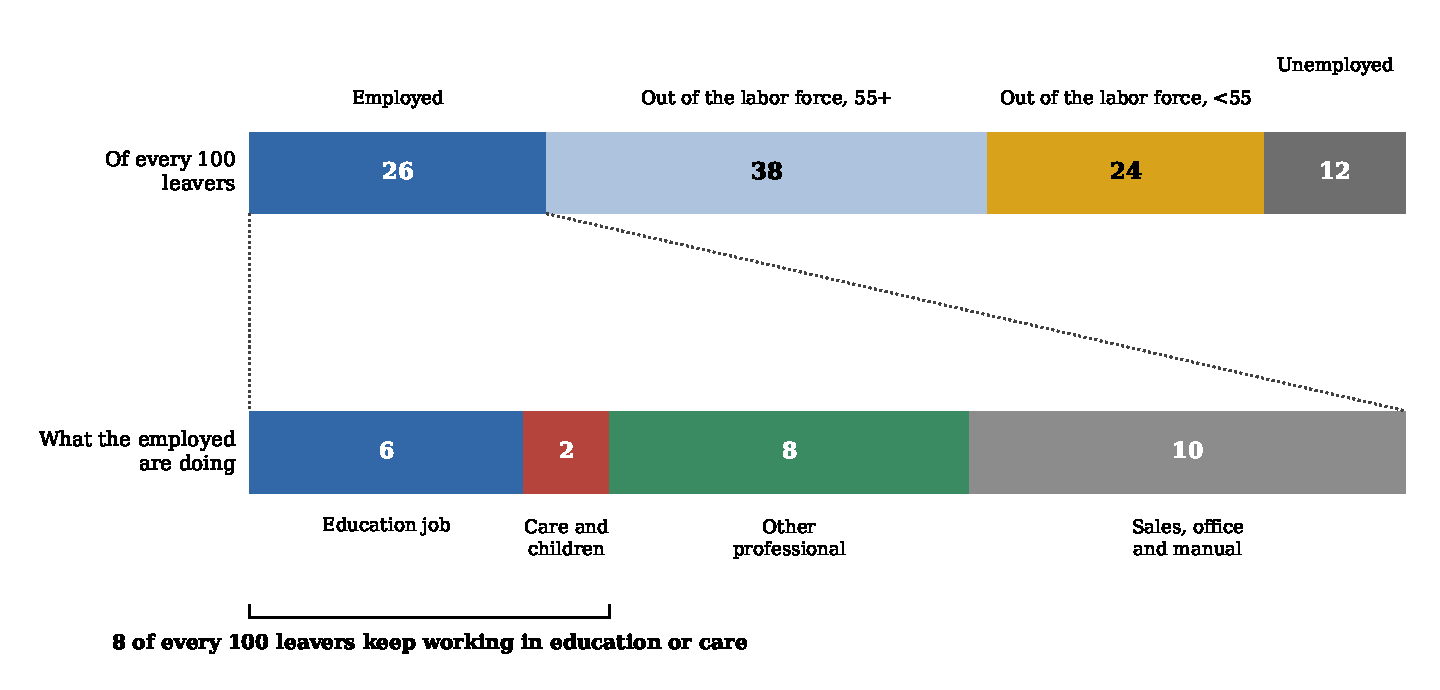
\includegraphics[width=0.9\linewidth]{figures/g3_flow100.pdf}
\caption{Destinations of Teachers Who Leave the Profession}
\fignote{\textit{Notes:} College-graduate leavers pooled over calendar
2015--2024, ASEC weights. Top bar: labor force status the March after
the teaching year; ``out of the labor force'' is split at age 55.
Bottom bar: the occupational destination of the 26 employed leavers,
rescaled to sum to their total. \textit{Source:} Author's calculations
from March CPS supplements.}
\end{figure}
\clearpage

\begin{figure}[H]
\centering
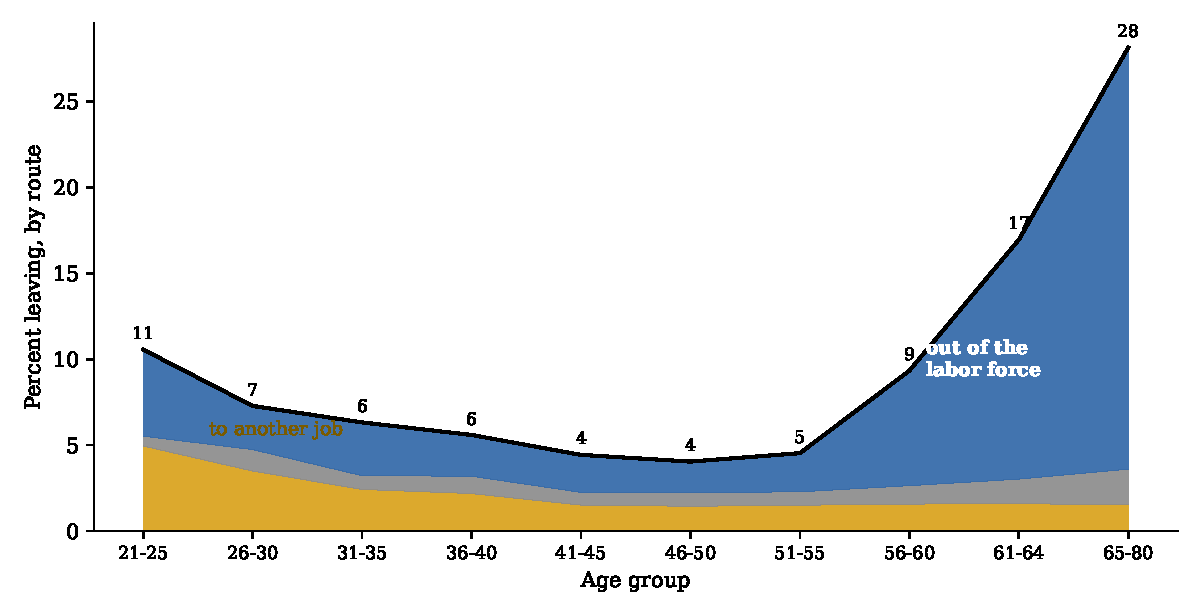
\includegraphics[width=0.9\linewidth]{figures/g4_routes_age.pdf}
\caption{Leaving Teaching by Age and Route}
\fignote{\textit{Notes:} College-graduate teachers pooled over
calendar 2015--2024, ASEC weights; ten age groups. The black line is
the total leaving rate; stacked areas decompose it into exits to
another job (gold), unemployment (gray), and out of the labor force
(blue). \textit{Source:} Author's calculations from March CPS
supplements.}
\end{figure}
\clearpage

\begin{figure}[H]
\centering
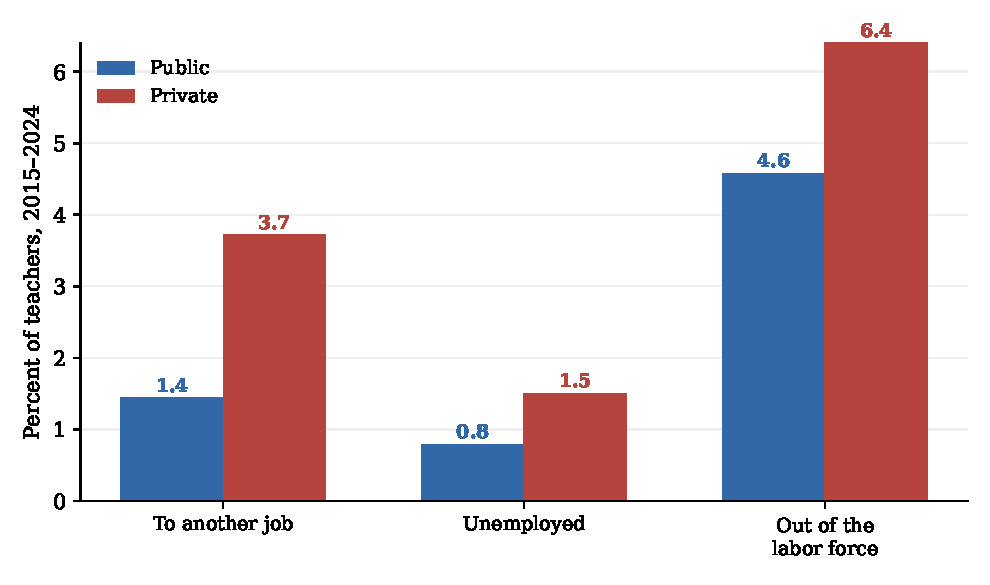
\includegraphics[width=0.62\linewidth]{figures/g10_sector_routes.pdf}
\caption{Exit Routes by School Sector}
\fignote{\textit{Notes:} Route-specific annual exit rates of
college-graduate teachers by sector of the last-year job
(class-of-worker: government vs.\ private), pooled 2015--2024, ASEC
weights. A private-school teacher who moves to a public school---or
vice versa---remains a teacher and is not a leaver here.
\textit{Source:} Author's calculations from March CPS supplements.}
\end{figure}
\clearpage

\begin{figure}[H]
\centering
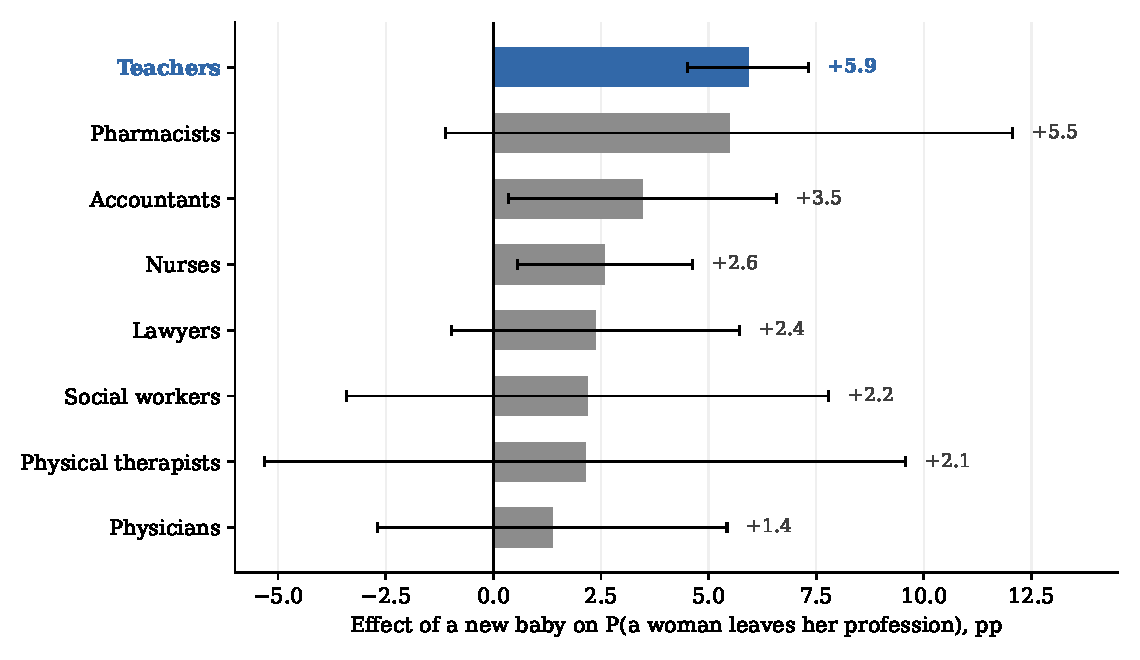
\includegraphics[width=0.82\linewidth]{figures/g8_newbaby.pdf}
\caption{The Effect of a New Baby on Leaving, by Profession}
\fignote{\textit{Notes:} Average marginal effect of a new baby (own
child aged 0 in the household) on the probability that a woman leaves
each profession, from profession-specific probits with age, age
squared, marital status, education, and year effects; whiskers are 95
percent confidence intervals. Solid bars are significant at 5 percent;
light bars are not. Samples pool 2010--2024. \textit{Source:} Author's
calculations from March CPS supplements.}
\end{figure}
\clearpage

\begin{figure}[H]
\centering
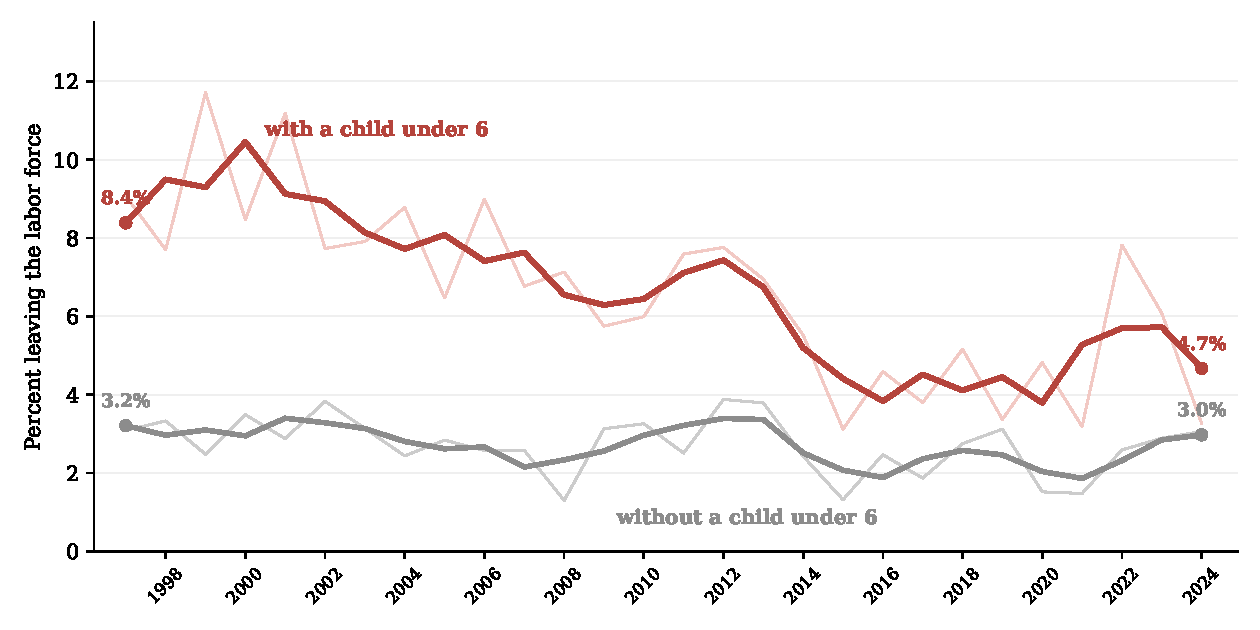
\includegraphics[width=0.92\linewidth]{figures/g9_mothers.pdf}
\caption{Labor Force Exit of Women Teachers, With and Without Young
Children}
\fignote{\textit{Notes:} Women teachers aged 22--45, college
graduates; annual probability of leaving the labor force (thin lines)
and centered 3-year averages (bold), separately for those with and
without an own child under 6 at home. Endpoint values printed.
\textit{Source:} Author's calculations from March CPS supplements,
survey years 1998--2025.}
\end{figure}
\clearpage

\begin{figure}[H]
\centering
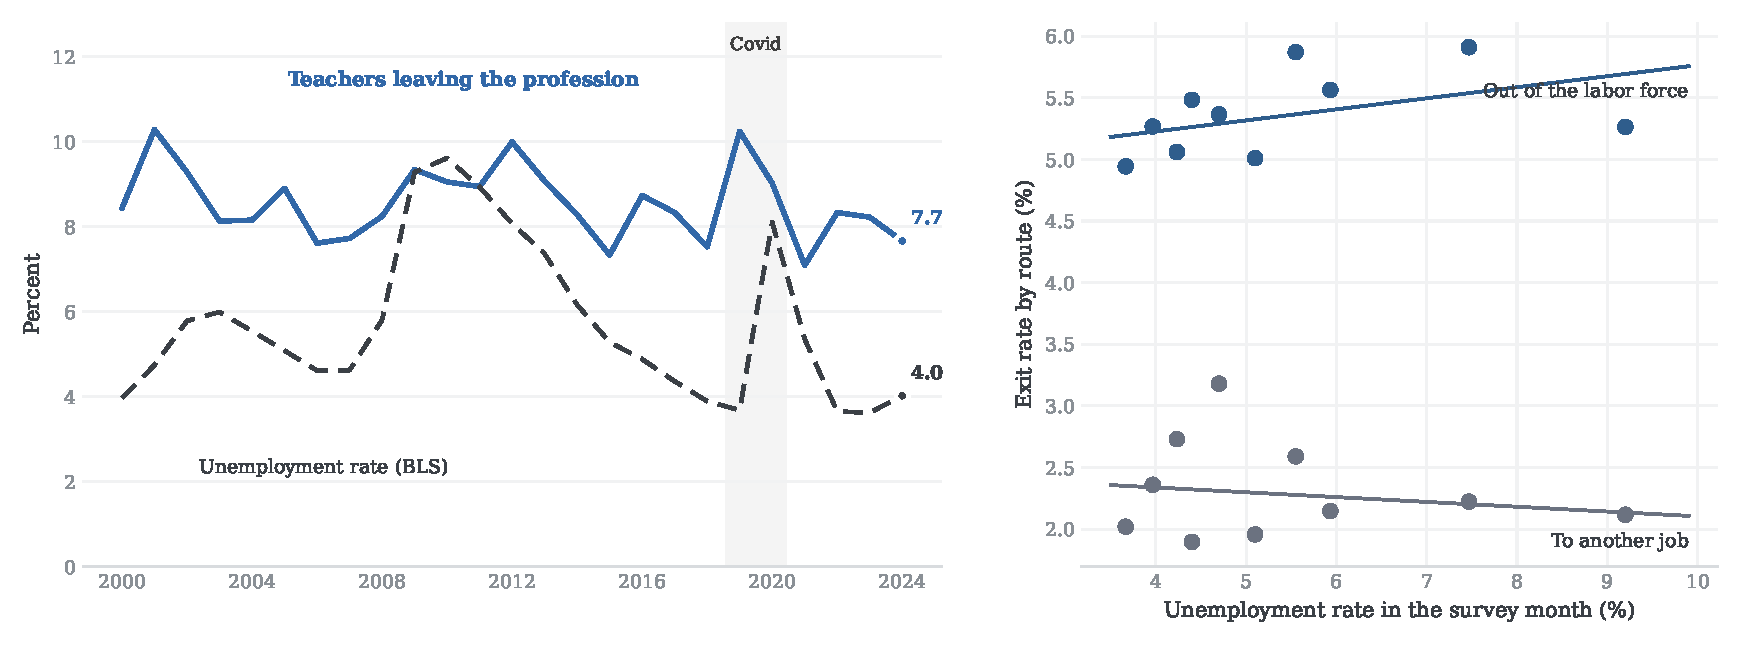
\includegraphics[width=\linewidth]{figures/n5_cyclicality.pdf}
\caption{Leaving Teaching and the Unemployment Rate, 1997--2024}
\fignote{\textit{Notes:} Left: the leaving series of Figure~2 (annual,
from calendar 2000) against the BLS national unemployment rate (annual
average). Right: binned scatter (deciles of the unemployment rate in
the survey month, March of $t{+}1$, when the exit is observed) of the
two labor-market routes, with OLS fits on the underlying annual data;
correlations are $-0.16$ (to another job) and $+0.29$ (out of the
labor force). Unemployment: BLS via FRED (\texttt{UNRATE}).
\textit{Source:} Author's calculations from March CPS supplements.}
\end{figure}
\clearpage

\begin{figure}[H]
\centering
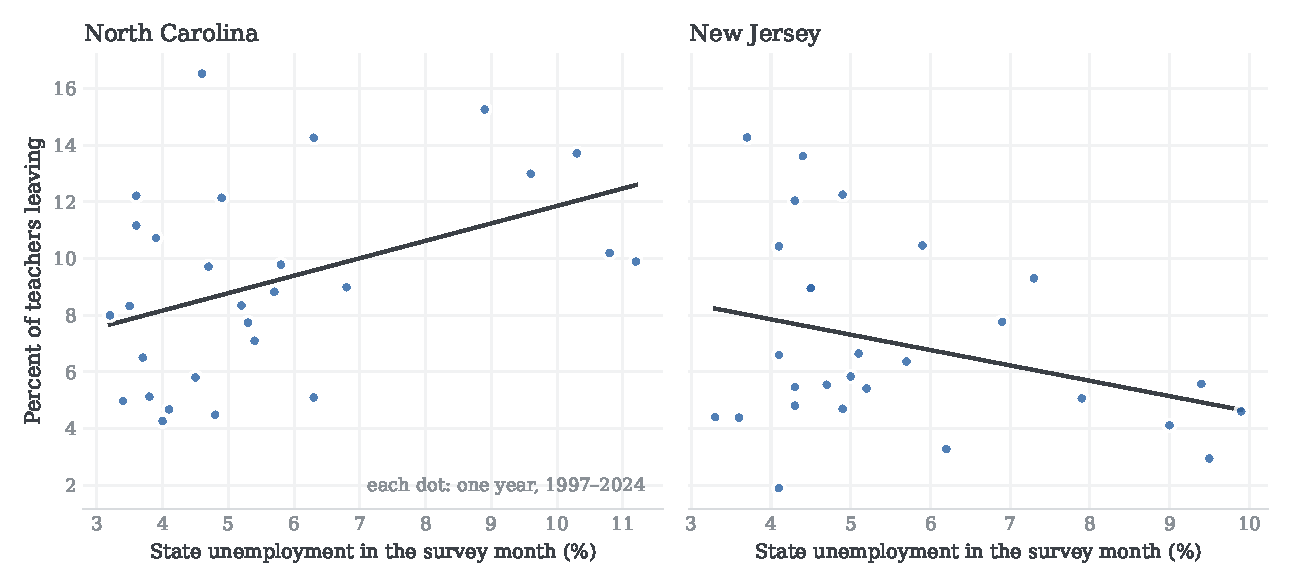
\includegraphics[width=0.85\linewidth]{figures/n5b_states_trio.pdf}
\caption{Leaving and State Unemployment: Two Examples}
\fignote{\textit{Notes:} Annual state leaving rates of
college-graduate teachers (dots; one per year, 1997--2024) against the
state unemployment rate in the survey month (BLS Local Area
Unemployment Statistics), with OLS fits. North Carolina and New Jersey
are shown as examples of the two signs; the full 51-state distribution
of slopes is in Figure~14. State of residence is recovered from the
household records of the raw files. \textit{Source:} Author's
calculations from March CPS supplements.}
\end{figure}
\clearpage

\begin{figure}[H]
\centering
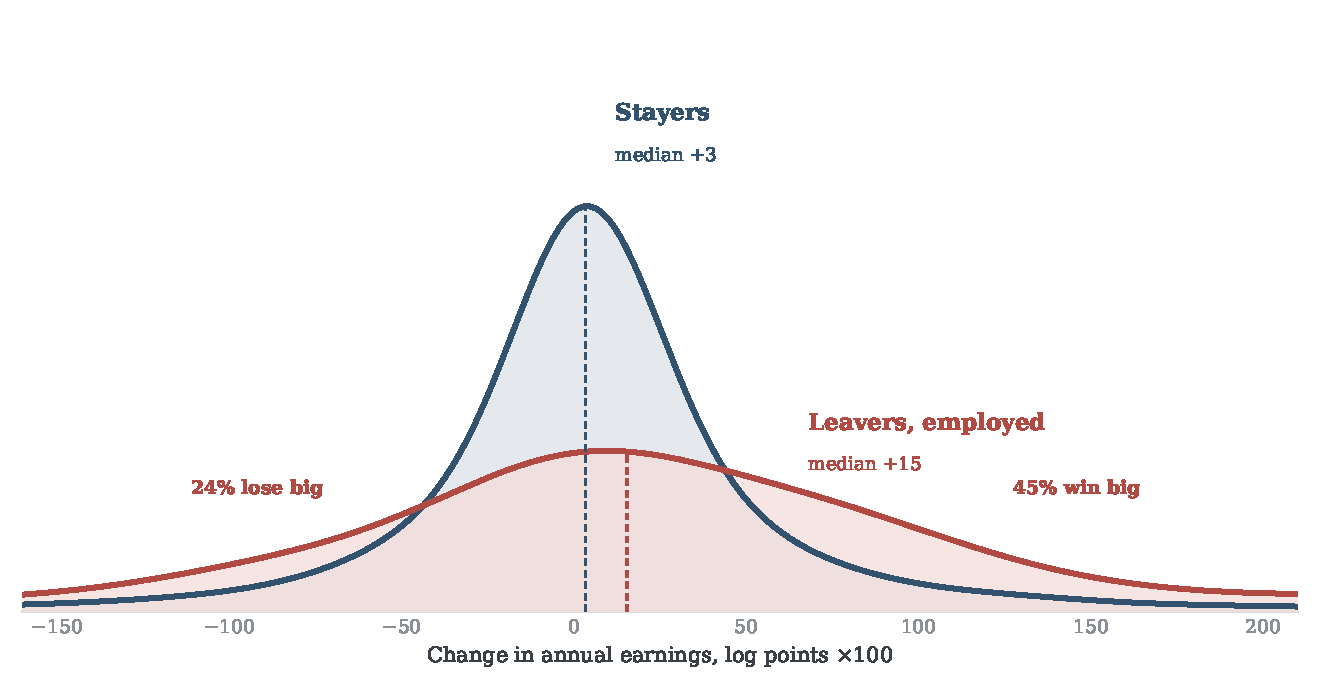
\includegraphics[width=0.9\linewidth]{figures/g5b_earnings_density.pdf}
\caption{The Distribution of Earnings Changes: Stayers and Leavers}
\fignote{\textit{Notes:} Kernel densities of the person-level change
in annual wage and salary earnings (log points $\times$100) between
the teaching year and the next, for teachers linked across consecutive
supplements (rotation-group links, survey years 2011--2025; identity
validated on sex and age). Navy: stayers (12,195 links; median $+3$).
Red: leavers employed the following year (225 links; median $+15$).
``Lose big''/``win big'' denote changes beyond $\pm$30 log points. The
sample conditions on positive earnings in both years; 47 percent of
all leavers report zero wage and salary earnings the following year.
Bandwidth 0.25. \textit{Source:} Author's calculations from March CPS
supplements.}
\end{figure}
\clearpage

\begin{figure}[H]
\centering
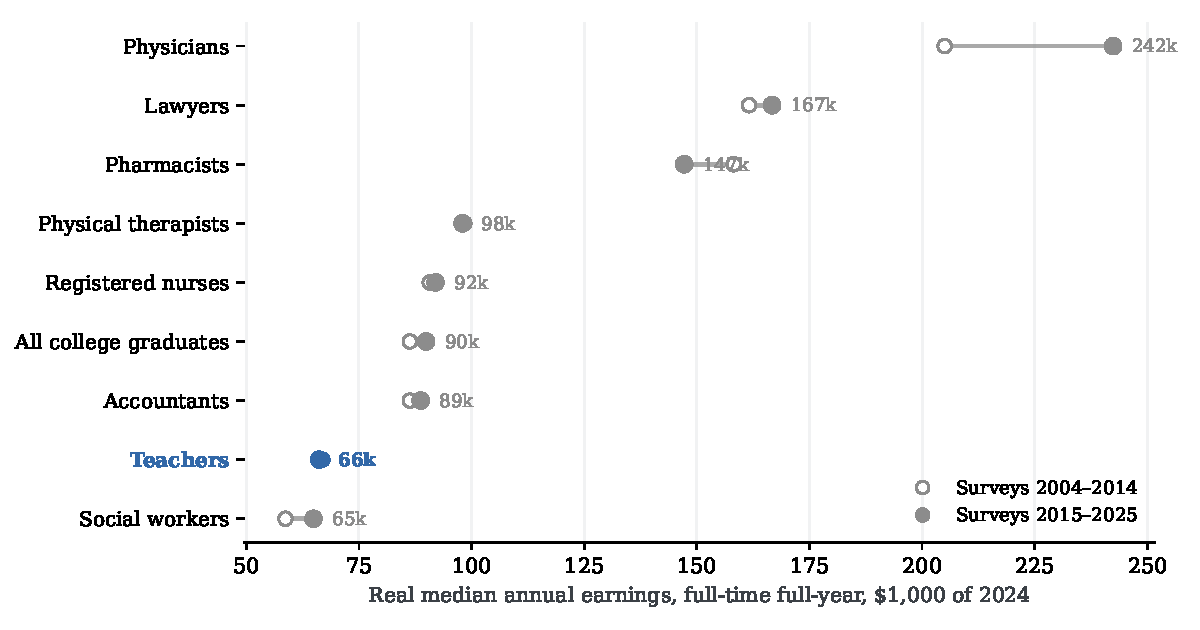
\includegraphics[width=0.85\linewidth]{figures/n6b_pay_windows.pdf}
\caption{Real Median Earnings by Profession, 2004--2014 and 2015--2025}
\fignote{\textit{Notes:} Weighted median annual wage and salary
earnings of full-time, full-year college graduates aged 25--60, in
each profession and overall, deflated to 2024 dollars with the CPI-U;
the two windows pool survey years 2004--2014 and 2015--2025. Filled
dots (with values): recent window. Occupation codes harmonized across
classification regimes. \textit{Source:} Author's calculations from
March CPS supplements; CPI: BLS via FRED.}
\end{figure}
\clearpage

\begin{figure}[H]
\centering
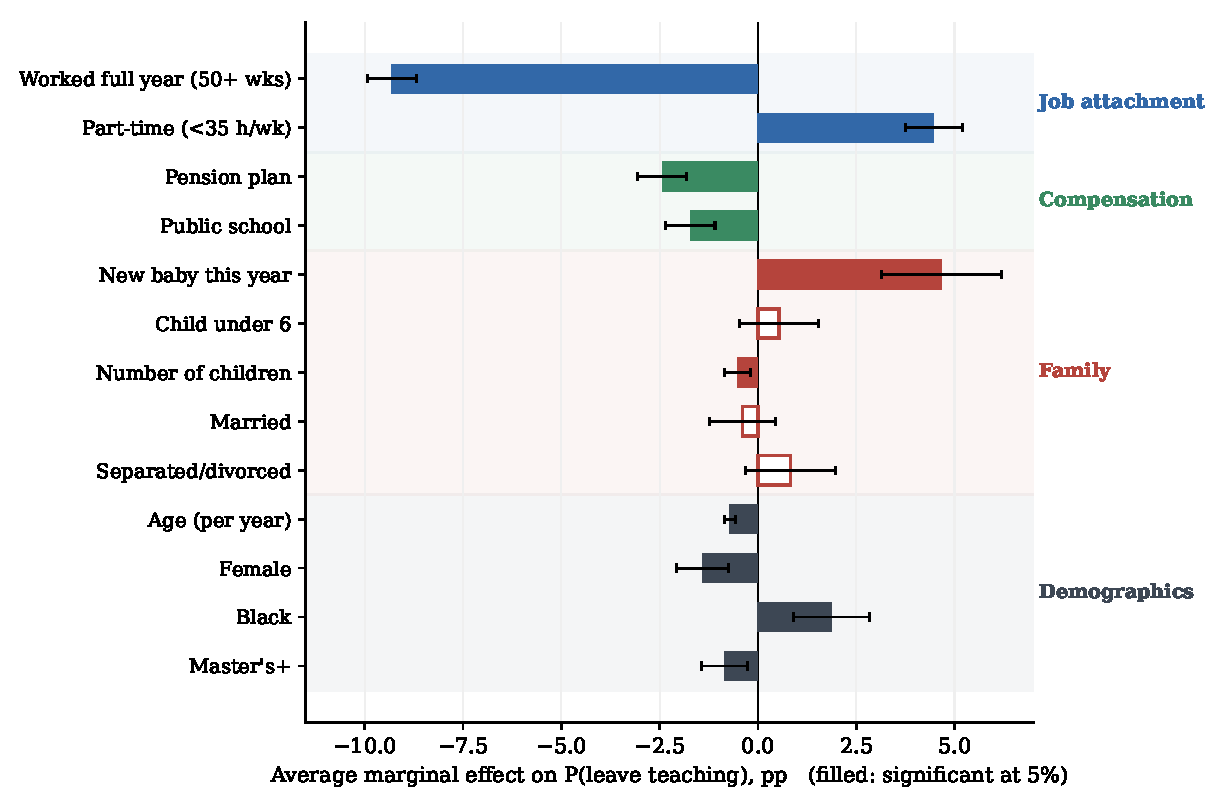
\includegraphics[width=0.8\linewidth]{figures/g6_ame.pdf}
\caption{Average Marginal Effects on the Probability of Leaving
Teaching}
\fignote{\textit{Notes:} Average marginal effects (percentage points)
on the probability of leaving teaching, from a probit on
college-graduate teachers pooled over calendar 2015--2024 with year
effects; whiskers are 95 percent confidence intervals; filled markers
are significant at 5 percent. ``Worked full year'' is 50+ weeks at the
last-year job; ``part-time'' is under 35 weekly hours. $n=28{,}900$.
\textit{Source:} Author's calculations from March CPS supplements.}
\end{figure}
\clearpage

\begin{figure}[H]
\centering
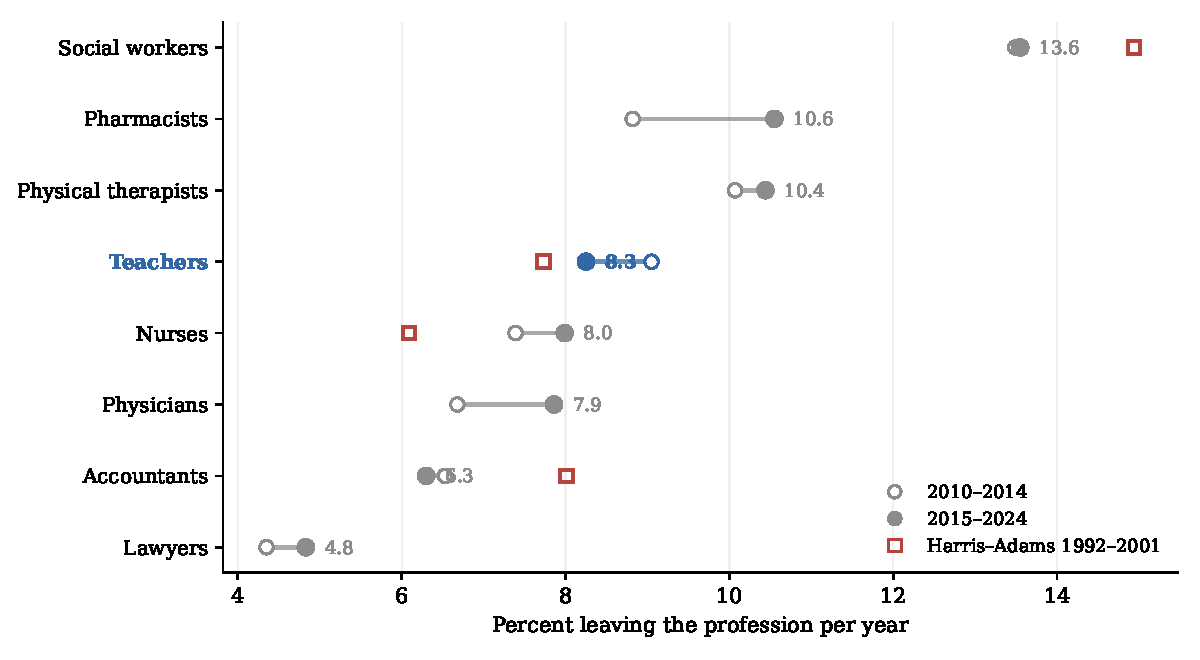
\includegraphics[width=0.85\linewidth]{figures/g7_professions.pdf}
\caption{Rates of Leaving by Profession, 2004--2014 and 2015--2025}
\fignote{\textit{Notes:} Annual rate of leaving each profession (same
route-based definition as for teachers, college graduates, ASEC
weights), pooled over survey years 2004--2014 (open) and 2015--2025
(filled, with values). Occupation codes harmonized across the 2002,
2010, and 2018 Census classification regimes. \textit{Source:}
Author's calculations from March CPS supplements.}
\end{figure}
\clearpage

% ================= appendix figures =================
\begin{center}{\large\bfseries Appendix Figures}\end{center}

\begin{figure}[H]
\centering
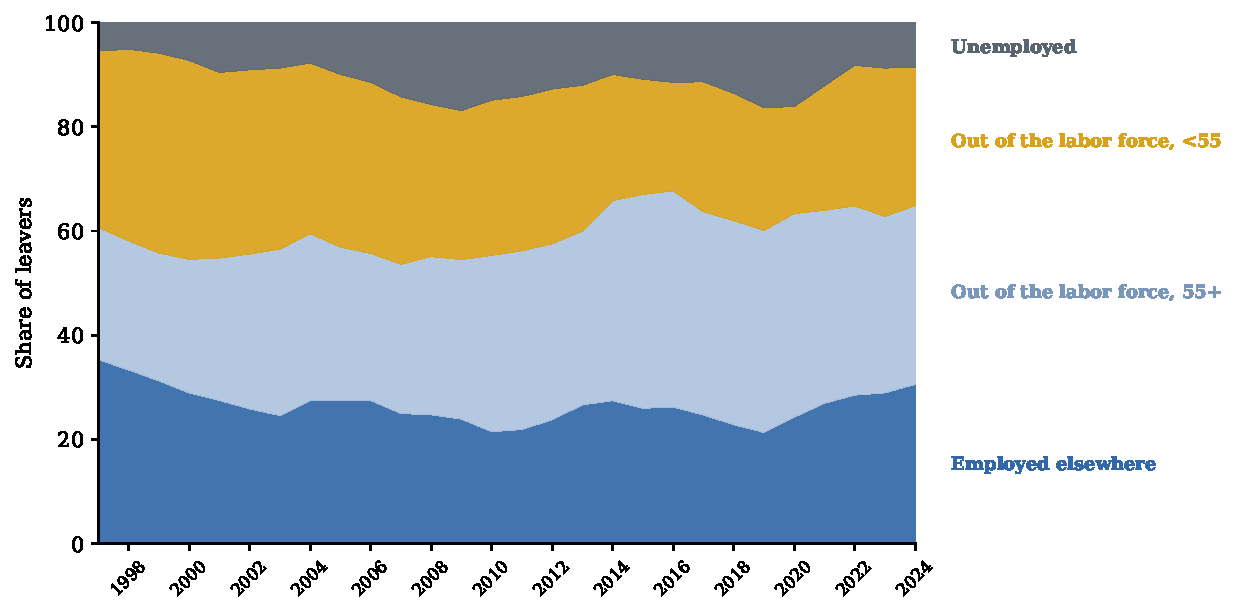
\includegraphics[width=0.9\linewidth]{figures/gapp_routes_evolution.pdf}
\caption{Route Composition of Leavers, 1997--2024}
\fignote{\textit{Notes:} Shares of college-graduate leavers by route
(3-year averages, renormalized to 100). The retirement-age share rises
from roughly a quarter to nearly forty percent; the young
out-of-labor-force (family) share falls symmetrically.
\textit{Source:} Author's calculations from March CPS supplements.}
\end{figure}
\clearpage

\begin{figure}[H]
\centering
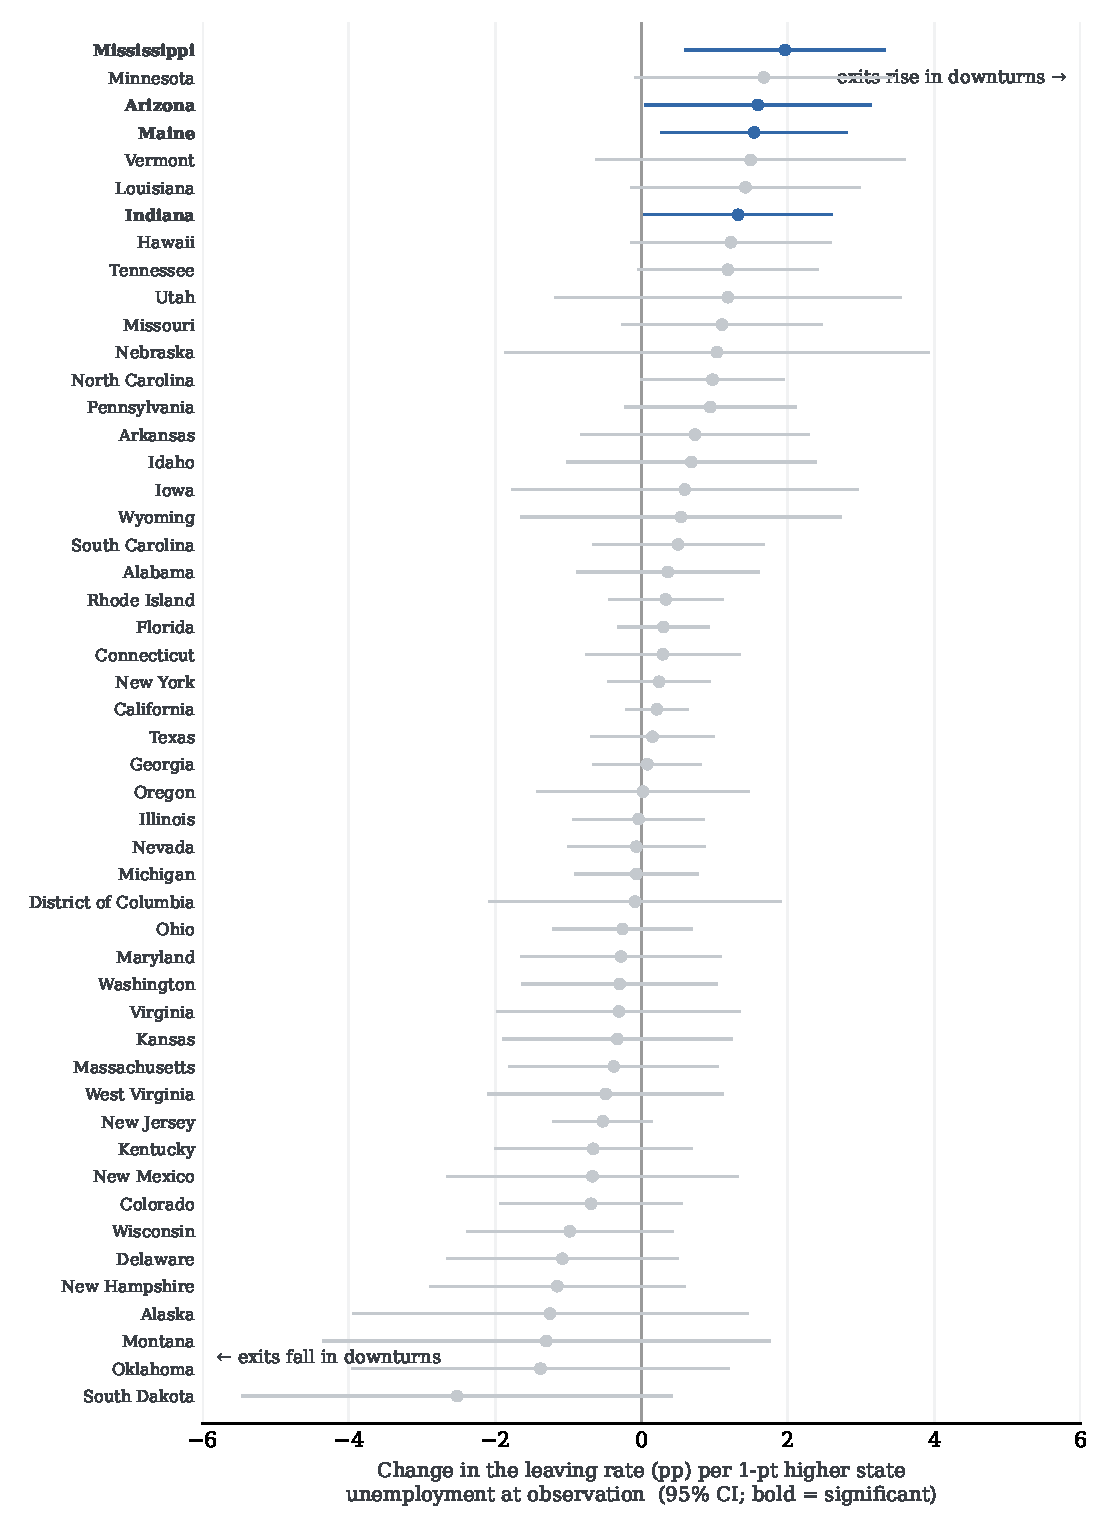
\includegraphics[width=0.62\linewidth]{figures/napp_state_cyclicality.pdf}
\caption{State-Level Cyclicality of Leaving, All 51 Jurisdictions}
\fignote{\textit{Notes:} Slope of a weighted linear probability model
of leaving on the state unemployment rate in the survey month,
estimated separately by state on all years 1997--2024; 95 percent
intervals, heteroskedasticity-robust. Bold: significant at 5 percent.
\textit{Source:} Author's calculations from March CPS supplements and
BLS LAUS.}
\end{figure}
\clearpage

\begin{figure}[H]
\centering
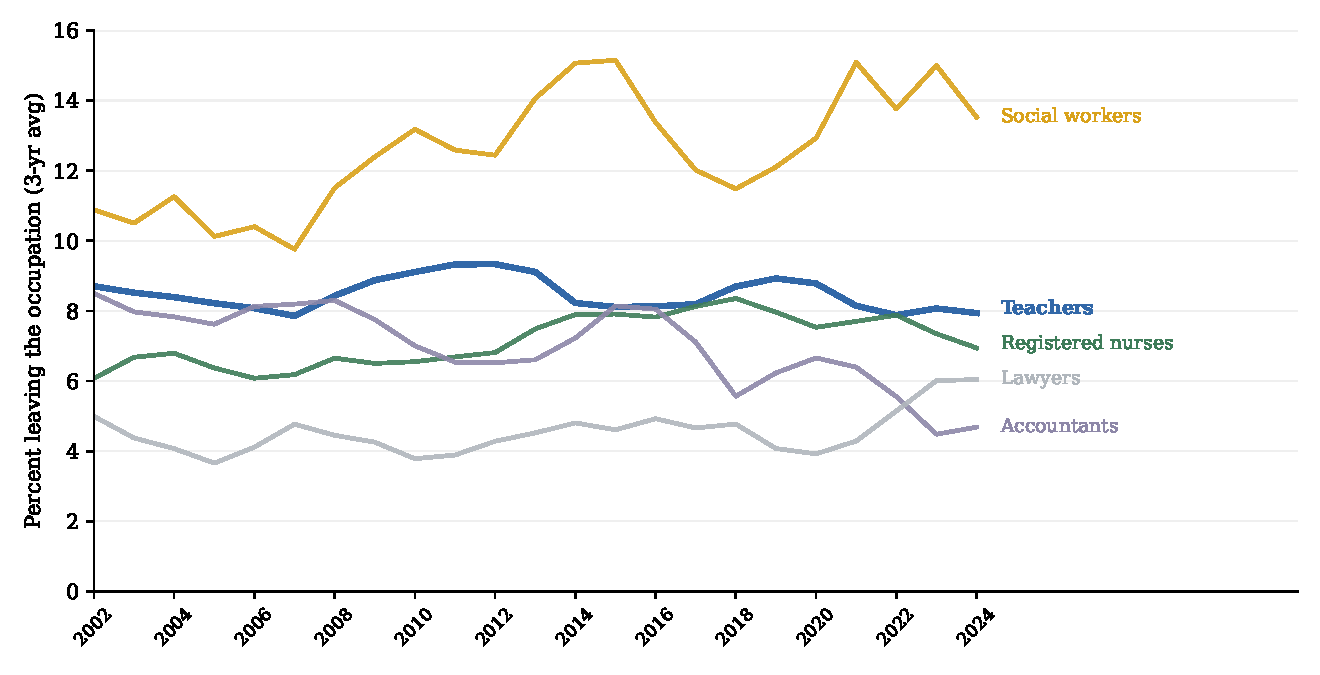
\includegraphics[width=0.9\linewidth]{figures/n6a_professions_series.pdf}
\caption{Leaving Rates in Five Professions, Annual Series}
\fignote{\textit{Notes:} Three-year averages of the annual
occupational leaving rate, college graduates, identical definitions
across professions; the window figures pool these series.
\textit{Source:} Author's calculations from March CPS supplements,
survey years 2003--2025.}
\end{figure}
\clearpage

\begin{figure}[H]
\centering
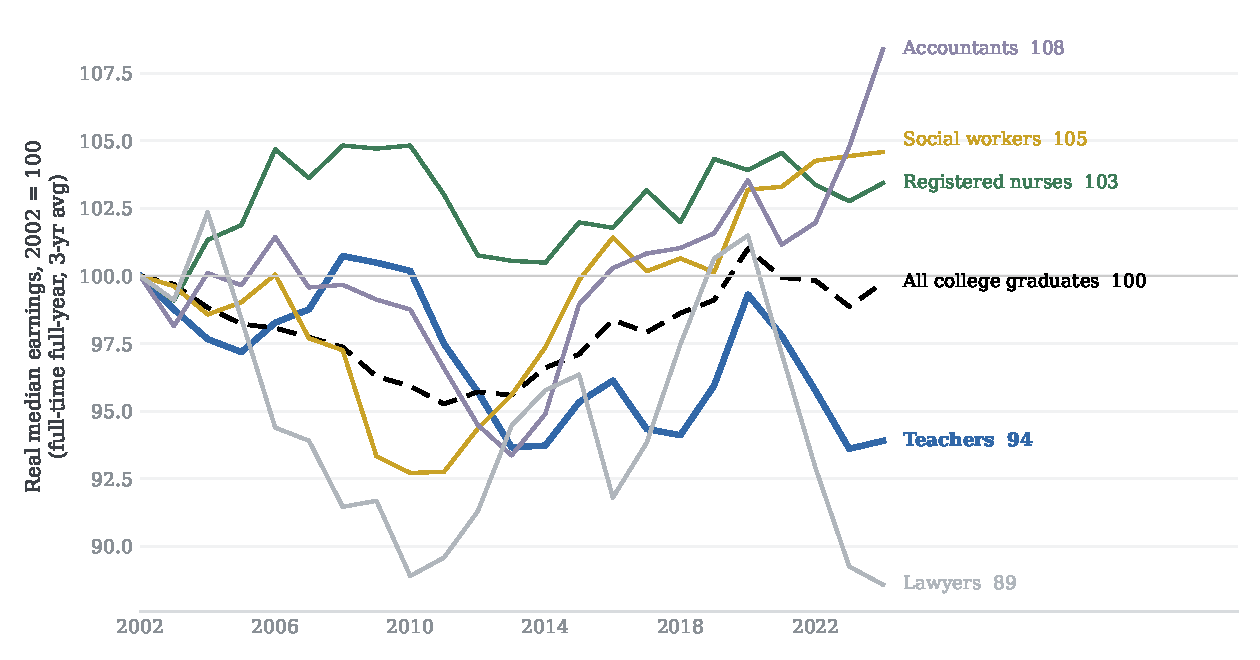
\includegraphics[width=0.9\linewidth]{figures/napp_pay_index.pdf}
\caption{Real Median Earnings by Profession, Indexed to 2002}
\fignote{\textit{Notes:} Real median annual earnings of full-time
full-year college graduates aged 25--60 by profession, CPI-U deflated,
indexed to 2002 = 100, 3-year averages; endpoint values printed.
\textit{Source:} Author's calculations from March CPS supplements.}
\end{figure}
\clearpage

\begin{figure}[H]
\centering
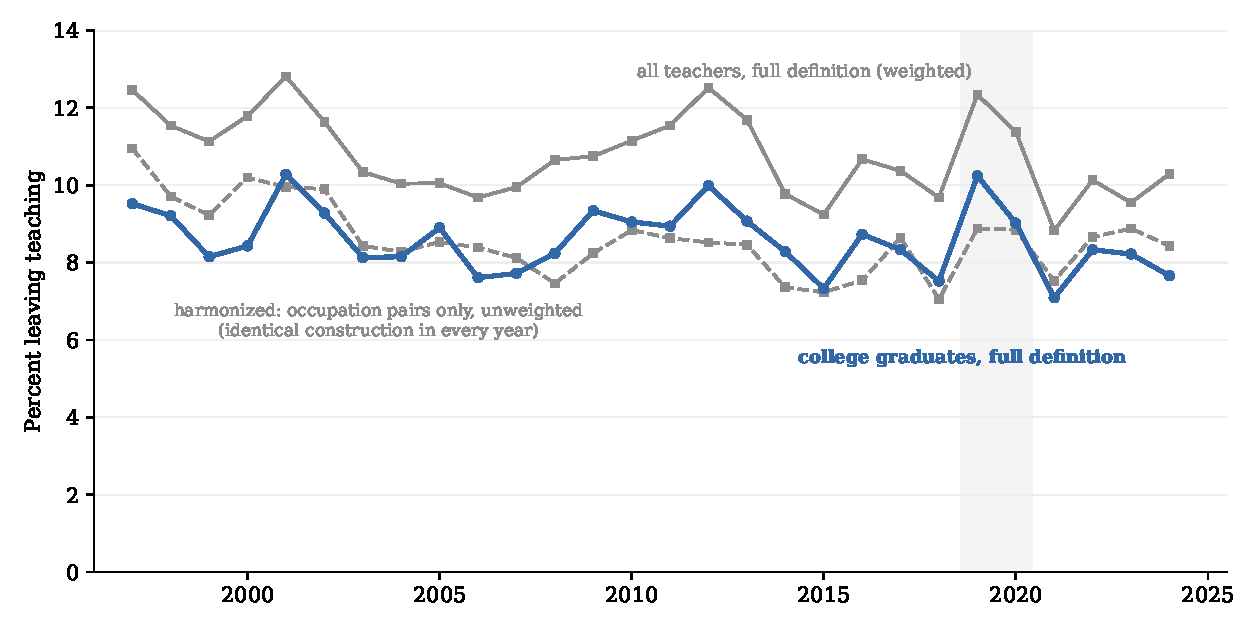
\includegraphics[width=0.92\linewidth]{figures/gapp_evolution_layers.pdf}
\caption{The Leaving Series under Alternative Definitions}
\fignote{\textit{Notes:} The baseline route-based college-graduate
series alongside the all-education series and the harmonized
occupation-pair-only construction. Levels differ by universe; profiles
coincide. \textit{Source:} Author's calculations from March CPS
supplements.}
\end{figure}
\clearpage

% ================= appendix tables =================
\begin{center}{\large\bfseries Appendix Tables}\end{center}

\begin{table}[H]
\centering\small
\caption{March Retrospective versus Linked-Panel Classification}
\begin{tabular}{lcccc}
\toprule
 & \multicolumn{3}{c}{March retrospective classification} & \\
\cmidrule(lr){2-4}
Linked-panel classification & Not a teacher & Stayed & Left & Total \\
\midrule
Stayer (teaches all 4 post months) & 198 & 7,911 & 67 & 8,176 \\
Leaver (teaches in none) & 1,018 & 10 & 257 & 1,285 \\
\midrule
Total & 1,216 & 7,921 & 324 & 9,461 \\
\bottomrule
\end{tabular}

\fignote{\textit{Notes:} Pooled linked sample, survey years
2011--2024. Rows: 4-month within-panel classification; columns: March
retrospective classification. \textit{Source:} Author's calculations
from CPS basic monthly files and March supplements.}
\end{table}

\begin{table}[H]
\centering\small
\caption{Leaving Rates and Routes: 1992--2001 versus 2015--2024}
\begin{tabular}{lcccccccc}
\toprule
 & \multicolumn{4}{c}{Harris \& Adams, 1992--2001} & \multicolumn{4}{c}{This paper, 2015--2024} \\
\cmidrule(lr){2-5}\cmidrule(lr){6-9}
 & All & Switch & Unemp. & Out LF & All & Switch & Unemp. & Out LF \\
\midrule
Teachers & 7.73 & 2.59 & 0.61 & 4.53 & 8.25 & 2.12 & 1.00 & 5.12 \\
Nurses & 6.09 & 1.68 & 0.86 & 3.54 & 7.99 & 3.66 & 0.81 & 3.53 \\
Social workers & 14.94 & 10.87 & 1.34 & 2.73 & 13.55 & 9.45 & 1.22 & 2.89 \\
Accountants & 8.01 & 4.10 & 1.55 & 2.36 & 6.30 & 1.79 & 1.18 & 3.32 \\
\bottomrule
\end{tabular}

\fignote{\textit{Notes:} Left block: Harris and Adams (2007),
Table~1, March CPS 1992--2001. Right block: author's calculations,
identical definitions, March CPS 2015--2024 (survey years 2016--2025).
All rates in percent per year. \textit{Source:} Harris and Adams
(2007) and author's calculations from March CPS supplements.}
\end{table}

\begin{table}[H]
\centering\small
\caption{Record Counts by Source}
\begin{tabular}{lcccc}
\toprule
Source & Survey years & Persons & Teacher-years & \shortstack{Teacher-years\\(BA+, 18+)} \\
\midrule
Machine-readable ASEC files & 2011--2025 & 2,585,797 & 54,620 & 45,296 \\
Fixed-width files, official layouts & 1998--2010 & 2,423,332 & 49,925 & 40,201 \\
\midrule
Total & 1998--2025 & 5,009,129 & 104,545 & 85,497 \\
\bottomrule
\end{tabular}
\fignote{\textit{Notes:} Teacher-years: longest job last year in a
K--12 teaching occupation. The baseline analysis universe is
college-graduate teachers aged 18+. Calendar-year coverage is
1997--2024. \textit{Source:} Author's calculations from March CPS
supplements.}
\end{table}
\clearpage

\begin{table}[H]
\centering\footnotesize
\caption{Descriptive Statistics: Teachers and Other College Graduates,
2015--2024}
\begin{tabular}{lcccc}
\toprule
 & Teachers, women & Teachers, men & All teachers & Other college workers \\
\midrule
\multicolumn{5}{l}{\emph{Demographics}} \\
Age (years) & 44.2 (12.8) & 44.9 (13.3) & 44.3 (12.9) & 44.1 (13.6) \\
Female & 100.0 & 0.0 & 76.0 & 48.7 \\
Black & 9.6 & 9.5 & 9.6 & 9.6 \\
Married & 66.6 & 67.7 & 66.9 & 62.6 \\
Child under 6 & 16.1 & 17.2 & 16.4 & 15.0 \\
Number of children & 0.8 (1.1) & 0.8 (1.1) & 0.8 (1.1) & 0.6 (1.0) \\
\multicolumn{5}{l}{\emph{Education}} \\
Master's degree or higher & 51.3 & 53.6 & 51.9 & 35.4 \\
\multicolumn{5}{l}{\emph{Job held last year}} \\
Government employer & 70.3 & 70.4 & 70.3 & 15.5 \\
Part-time (<35 h/wk) & 15.2 & 11.4 & 14.3 & 13.5 \\
Full year (50+ weeks) & 71.1 & 74.8 & 72.0 & 85.0 \\
Pension plan at work & 66.4 & 67.3 & 66.6 & 46.1 \\
Wage earnings, median (\$) & 50,000 & 58,000 & 52,000 & 70,000 \\
\multicolumn{5}{l}{\emph{Transitions}} \\
Leaves teaching within a year & 7.9 & 9.1 & 8.2 & -- \\
Person-years (unweighted N) & 22,097 & 6,785 & 28,882 & 277,364 \\
\bottomrule
\end{tabular}

\fignote{\textit{Notes:} Weighted means; standard deviations in
parentheses for continuous variables. Wage earnings are medians,
current dollars, conditional on positive earnings. ``Leaves teaching''
is undefined for non-teachers. \textit{Source:} Author's calculations
from March CPS supplements.}
\end{table}

\begin{table}[H]
\centering\footnotesize
\caption{Robustness of the Attrition Model}
\input{tables/probit_robustness}
\fignote{\textit{Notes:} The dependent variable is an indicator for
leaving teaching, scaled so that coefficients are percentage points.
Column 1 reports baseline probit average marginal effects, calendar
2015--2024, with year effects, unweighted. Column 2: linear
probability model, ASEC weights, heteroskedasticity-robust standard
errors. Column 3: logit average marginal effects. Column 4: weighted
linear probability model with state and year effects. Column 5: probit
on the full 1997--2024 window. Column 6: weighted linear probability
model with the occupation-pair definition of leaving. Standard errors
in parentheses.\starlegend}
\end{table}
\clearpage

\begin{table}[H]
\centering\footnotesize
\caption{The Attrition Model in Subsamples}
\input{tables/probit_subsamples}
\fignote{\textit{Notes:} Linear probability models of leaving teaching
(percentage points) estimated separately by subsample, with year
effects, ASEC weights, calendar 2015--2024;
heteroskedasticity-robust standard errors in parentheses. ``--'' marks
regressors without variation in the subsample.\starlegend}
\end{table}

\begin{table}[H]
\centering\small
\caption{Paid Family Leave and the Birth-Year Exit}
\begin{tabular}{lc}
\toprule
 & Leaves teaching \\
\midrule
New baby & 6.98*** \\
 & (0.82) \\
New baby $\times$ paid family leave & $-$2.87* \\
 & (1.54) \\
Paid family leave active & 0.04 \\
 & (0.30) \\
\midrule
State and year effects & Yes \\
Demographic controls & Yes \\
Observations & 77,883 \\
Births under active programs & 268 \\
\bottomrule
\end{tabular}
\fignote{\textit{Notes:} Weighted linear probability model of leaving
teaching (percentage points) on an indicator for a new baby,
interacted with an indicator for the state having an active paid
family leave program in the teaching year. First full benefit years:
California 2005, New Jersey 2010, Rhode Island 2014, New York 2018,
Washington 2020, District of Columbia and Massachusetts 2021,
Connecticut 2022, Oregon 2024. Standard errors, clustered by state, in
parentheses.\starlegend}
\end{table}

\end{document}
